\documentclass[a4paper,10pt]{article}
\usepackage[utf8]{inputenc}


\begin{document}



\paragraph{Openlayers} \footnote{Quelle: \cite{ol3begGuide}}

\begin{itemize}
 \item Eine Karte in OL setzt sich aus folgenden Elementen zusammen
 \begin{description}
  \item [ol.Map]   Das zentrale Element der karte; hier läuft alles zusammen; dies representiert die gesamte Karte
  \item [ol.control.Control] Elemente die über sichtabe UI Elemente die Interaktion mit der Karte erlauben
  \item [ol.interaction.Interaction] Erlaubt eine Interaktion mit der Karte mit Gesten, Klicks und Tastatureingaben
  \item [ol.layer.Base]  Layers die auf die Map gezeichnet werden können
  \item [ol.Overlay] Elemente die via HTML auf der Karte gezeichnet werden können
  \item [ol.View] Representiert die Sicht auf die Karte. Den Ort und das Zoomlevel.
 \end{description}
\item Elemente sind strickt objektorientiert. 
\item Alles erbt von Observable\footnote{siehe Figure \ref{fig:ol.objektstruktur}}
\item Alles bis auf Interaction erbt von ol.Object
\end{itemize}

\begin{figure}[h!]
 \centering
 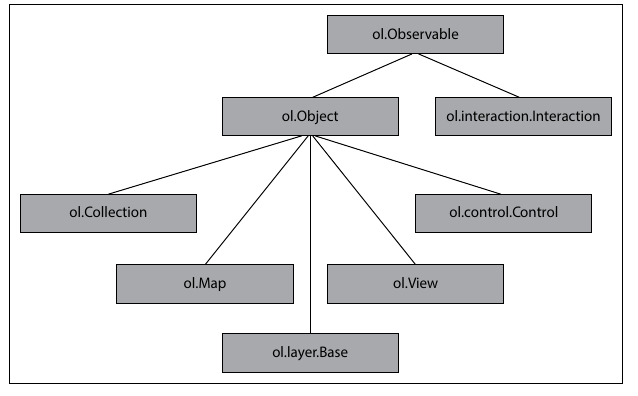
\includegraphics[width=\textwidth]{pix/ol_objektstruktur.png}
 % ol_objektstruktur.png: 638x396 px, 96dpi, 16.88x10.48 cm, bb=0 0 478 297
 \caption{Darstellung der Objektstruktur in Openlayers}
 \label{fig:ol.objektstruktur}
\end{figure}



\paragraph{Bootstrap}

\paragraph{SQLAlchemy}\label{par:anforderungen-SQLAlchemy}

SQLAlchemy kennt zwei Formen der Ausführung. Zum einen gibt es eine eigene Query sprache um mithilfe der Models Daten aus der Datenbank zu fischen. Zum  anderen gibt es die Möglichkeit SQL direkt auszuführen. Trotz der unsicherereren Handhabung wurde sich für SQL entschieden.  Somuit ist sichergestwellt, dass die gesamte Abfrage komplet in einer Tabelle aus der Datenbank gelesen wird. Die Query Logiuk hätte eine weit höhere Transaktionskosten. Diese würde jeden Wert einzeln aus der Datenbank picken.  %TODO Recherche: gibt es keine Möglichkeit auch mit SQLAlchemy Qeuries die gesamte Table abzuholen?  -- denke doch!

\end{document}


\subsection{Motivation}

Durch das weltweite vernetzen unserer Computer und der damit verbundenen Aggregation der Daten, haben wir die größte Ansammlung von Wissen in der Geschichte unseres Planeten erreicht.
Trotz dieser enormen Menge an Fakten und schieren Menge an potenziellem Wissen scheint sich in der letzten Zeit eher eine Abwendung vom Wissen und der damit verbundenen Anstrenung, neues zu lernen und erlentes durch eine Evidenzprüfung zu unterziehen, zu vollziehen. (QUELLE)

\subsection{Zielsetung}

Ziel dieser Arbeit ist es, die Entwicklung eines Pörototyps zur einfachen Betrachtung der Daten des Argo Projektes zu beschreiben und deren Ablauf darzustellen.

\subsection{Struktur der Arbeit}

